\subsection{O Problema do Clique}

Um clique em um grafo G não orientado é um subconjunto C de vértices tal que, para cada $v$ e $w$ em C com $v \neq w$, ($v$,$w$) é uma aresta.
Para um grafo não orientado G e um inteiro $k$ como entrada, decidir se há um clique em G de tamanho mínimo $k$ \cite{goodrichprojeto}.

O problema do clique é NP. Pois podemos verificar se existe no mínimo $k$ vértices em C e também se há uma aresta para cada par de vértices em C, em tempo polinomial. Para provar que o problema do clique é NP-Completo basta reduzir o problema \textit{vertex cover} ao problema do clique \cite{HOPCROFT1974}.

$Prova$ Dado um grafo G = (V, A), onde V são os vértices e A as arestas e sendo (G, $k$) uma instância do problema \textit{vertex cover}, também levando em consideração o complemento $\bar{G}$ deste grafo, que possui o mesmo conjunto do grafo G mas, aresta($v,w$) com $v \neq w$ se e somente se ($v,w$) não estiver em G. Podemos definir o parâmetro $k$ como n - $k$, onde o $k$ é um parâmetro inteiro para o \textit{vertex cover}. Esta construção pode ser executada em um tempo polinomial e funciona como uma redução, visto que $\bar{G}$ detem um clique de tamanho mínimo $n-k$ se e somente se G tiver uma cobertura de vértices com tamanho máximo $k$.\cite{goodrichprojeto}

\begin{figure}[H]
	\centering
	\label{fig1}
	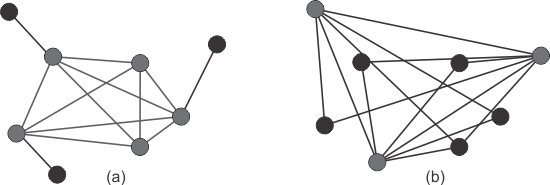
\includegraphics[scale=2]{./figuras/figClique.png}
	\caption{Um grafo G ilustrando a prova que o problema do Clique é NP-Difícil. (a) ilustra o grafo G com os vértices de um clique de tamanho 5 pintados na cor cinza. (b) mostra o grafo $\bar{G}$ com os vértices de um clique de tamanho 3 coloridos de cinza. \cite{goodrichprojeto}}
\end{figure}
